
\documentclass[11pt, letterpaper]{article}

\title{Push: a DISC shell}
\author{Noah Evans(to be considered for the best student paper award)\\
IBM Research\\
Nara Institute of Science and Technology\\
noah-e@is.naist.jp\\\\
Eric Van Hensbergen\\
IBM Research\\
ericvh@us.ibm.com\\
}

\usepackage{fullpage}

\usepackage{graphicx}

\date{}

\begin{document}

\maketitle

\pagebreak

%\begin{abstract}
%
%Pipes were a major advance in software engineering, allowing the composibility of previously isolated programs regardless of programming language. With the move to Data Intensive Supercomputing there is a similar trend towards the use of pipelines. Systems define graphs of processes, the edges of the graphs representing pipes and their vertices represent computation on a system.  With these systems and a new class of languages built on top of them researchers can solve "pleasantly parallel" problems more quickly without worrying about explicit concurrency.
%
%This approach is powerful and appropriate for many problem types. However as of yet none of these systems have been able to recapture the conceptual simplicity and ease of use of UNIX pipelines as implemented by the shell. We have implemented a shell using Data Intensive SuperComputing(DISC) principles, PUSH, which contains built in operators to provision and connect virtual and/or physical OS instances.  Process interconnections are composed using synthetic file systems, pushing the distributed complexity into the operating system and out of middleware. In this paper we explore the motivations, design and implementation of the PUSH shell showing how it can be used to solve many DISC problems. Finally we show how the system can be used with two current utility computing systems, IBM's kittyhawk and Amazon's EC2 to transparently interconnect and run DISC processes using only the terseness and expressivity of the shell.
%
%\end{abstract}

\renewcommand{\topfraction}{0.85}
\renewcommand{\textfraction}{0.1}



\section{Introduction}

With the advent of huge publicly available data sets such as sensor networks, online transactions, and web data, users are now able to work with much more data than ever before. However it is also impossible to deal these data sets in a reasonable amount time and economically even using the most powerful isolated machines. This problem is described in depth in \cite{barroso2003wsp}.

Data Intensive Scalable Computing(DISC)\cite{bryant2007dis} has become a standard tool to solve research problems using these datasets. By dividing the data into structured records and then distributing these records onto large sets of computational resources users can solve previously intractable problems using large clusters of commodity hardware. Correspondingly there has been a proliferation of different languages and systems allowing the provisioning, filtering, distribution and aggregation of petabytes of information over a variety of systems.

At the lowest level these DISC systems are implemented using platforms like Google's MapReduce\cite{dean2008msd}, Microsoft's Dryad\cite{isard2007ddd} and Apache/Yahoo's Hadoop\cite{bialecki:hfr}. These platforms provide a job scheduler, work partitioning and execution. Built on top of these systems are languages like Sawzall\cite{pike2005idp}, DryadLinq\cite{yu2008dsg} and Pig Latin\cite{olston2008pln} which allow the expression of DISC jobs and workflows without the bookkeeping and verbosity of manipulating and programming for DISC systems directly.

These languages provide automated control flow(typically matched to the archicture of the underlying system) and channels of communication between systems, but none of these languages match the terseness and simplicity of the UNIX shell model (e.g. 'sort | uniq -c') which can compose a number of smaller programs into a coherent workflow to solve more complicated problems quickly. In addition these static workflows are tied to the systems that they are written on. This makes solutions written for one DISC system inherently incompatible with other systems, tying solutions to a particular middleware, workflow and language.

The UNIX programming environment was designed to get around many of these problems. By providing a standard set of tools at the systems level UNIX standardized the ways programs were instantiated(fork()) and communicated(through device independent file descriptors).  This standardization allowed compiled programs to be portable between systems various Unices as long as programs adhered to the standard UNIX interface(codified by POSIX), paid attention to architectural details(like endianess) and reading and writing from specified file descriptors, UNIX programs were portable and consistent between systems. 

Adding to this portability standardizing upon certain io ports had an even greater advantage--pipes. Programs read from standard input and write to standard output. By changing the targets of these standard  IO ports programs could be composed with one another through pipelines, which rerouted a program's output descriptor into the input descriptor of another, allowing programs to work together in streams \emph{with no explict knowledge of this chaining built into the program itself}(the initial idea for the pipes concept was described in \cite{mcilroy1964paf}). 

Contrast this with the current way of writing solutions for DISC systems , which ---despite being written on a POSIX system--- use vastly different problem solving architectures and methods in the system. By implementing their systems as middleware on top of a UNIX they lose UNIX's advantages.  To port tools from one DISC system to another users must to completely reimplement tools, quite often with a different philosophy and data model to get what they want. Many research groups, notably \cite{isard2007ddd} have noticed the discrepency and have attempt to make it possible to use preexisting sequential code to solve problems in a DISC manner.

However these systems are still cumbersome. Dryad's workflow creation program requires the user to manually specify and manipulate graphs of executable programs via a GUI. Users place "vertices" which are connected by communications "channels"(the edges of the graph) to specify the data flow between processes. Because users have to compose and connect their processes graphically a user has to meticulously plan and implement the distribution of their computation.

Comparing the dryad process of creating a manual graph of input and output communication to the traditional writing of a UNIX shell script. Users use a vocabulary of components, scripts, executables and shell commands, which users can invoke quickly and then iteratively to refine the resulting workflow until a desirable solution is reached.

However the Dryad approach is appropriate to the current context of DISC program writing, where the systems used are extremely large, expensive and set preexisting special purpose computation resources shared between many users. The cost of CPU time makes programmer time less important, leading to a situation where ad hoc iterative solutions are a waste of system and resource time. \cite{pike2005idp} describes Google's solutions to problem with Sawzall.

However with the advent of systems like EC2\cite{amazon:aec}, individuals can create ad hoc DISC systems without the same massive overheads that have traditionally kept DISC systems the domain of companies with large resources like Google and Microsoft.

Now users find themselves in situations where they need the ability to solve a problem by coordinating a set of systems but the complexity and power of an optimized DISC system are unnecessary. 

Currently users do much of this distribution manually with a sequence of remote execution commands like ssh(1) but this process loses much of the original context of the originating system's environment, file system and control flow. Files may need to be resynchronized on new instances and the user has no standard way of collating data short of writing data to local files on each instance and copying those files back to a central server or using a common file server.

These two situations, over complex DISC systems and the difficult creation and use of ad hoc systems leaves users at an impasse. They can deploy huge DISC systems that work within certain domain and company specific languages or use cumbersome approaches which are difficult to deploy for ad hoc DISC solutions. 

With the ready availability of cheap, easy to provision cluster resources, we feel the time is ripe for the development of a more generalized framework for DISC computing that leverages the dynamic availability of resources, facilitates the use of any language or runtime, and has the simple, terse, composability of the UNIX shell. Specifically we wish to create a system that dynamically provisions computation and then interconnects it automatically while still being language independent and retaining a common context between systems.

Furthermore we argue that this kind of solution is better implemented at the systems rather than the middleware level. By implementing DISC systems at the systems level you provide a standard set of resources that allow the user to build DISC applications, like high level DISC languages, in a composable and middleware independent manner. 

\section{Overview}
\begin{figure}[htp]
\centering
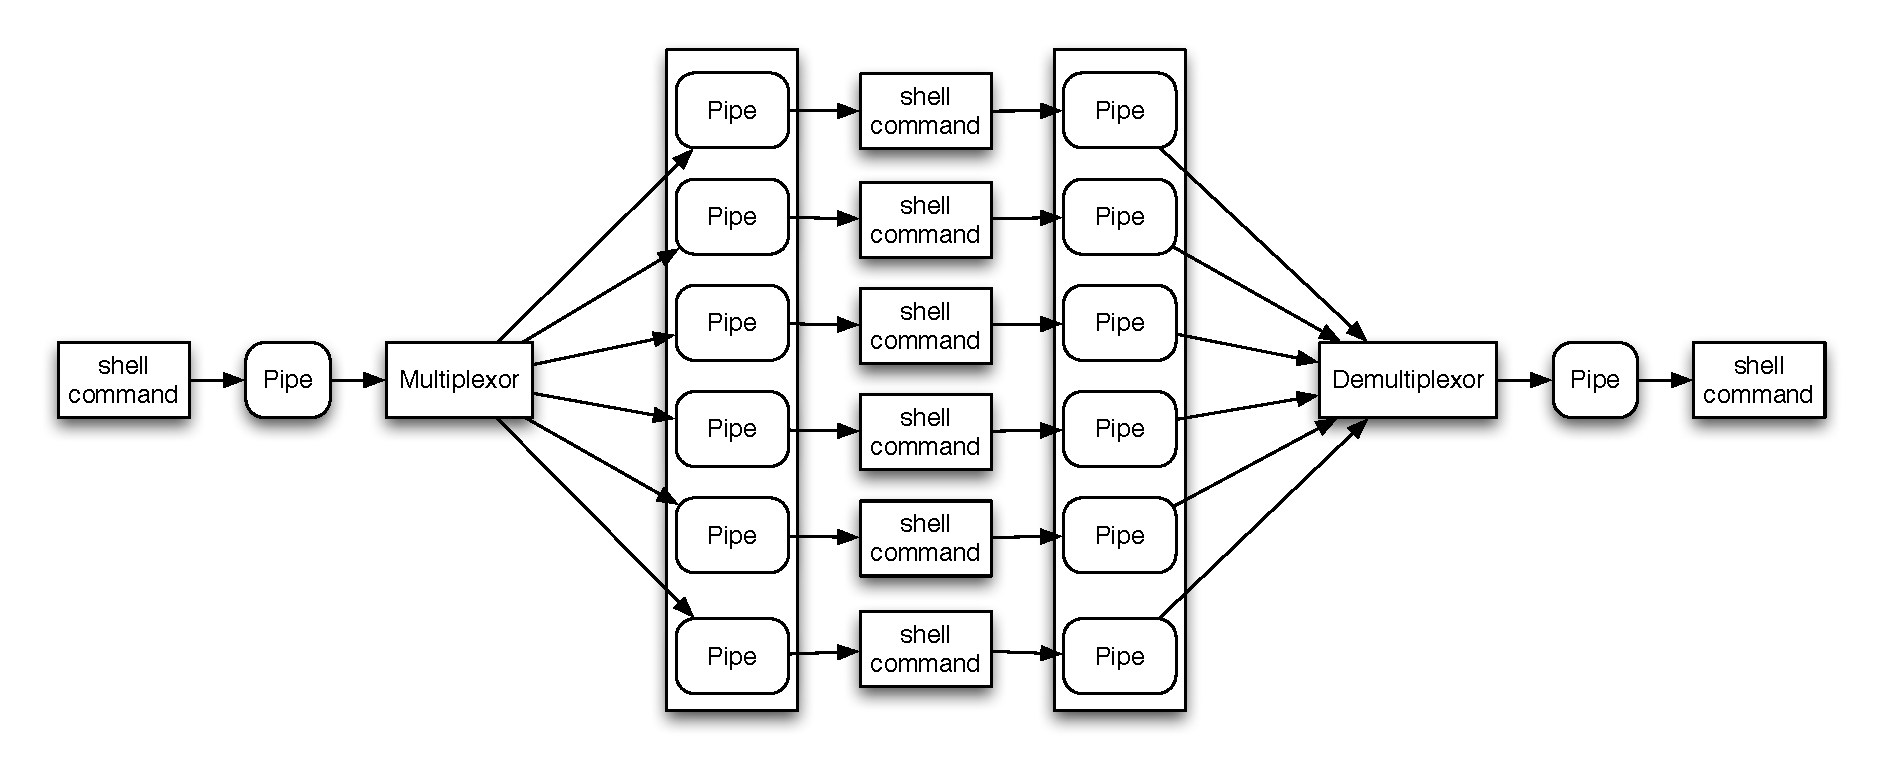
\includegraphics[width=4.5in]{pipestruct.eps}
\caption{The structure of the Push shell. Push implements a new form of multiplexed pipelines which all the distribution of record based output to multiple threads of control. This data is first "Fanned out" to multiple pipes by a multiplexor and then it is subsequently "Fanned in" by a de-multiplexor}\label{fig:pipestruct} 
\end{figure}
To achieve this ease of portability and terseness we have created a scalable, portable DISC shell, Push, using calls for dynamic provisioning and a pipe abstraction which makes it possible to do many to one and one to many communication. 

One of the principle advantages of the UNIX shells is that they allow the composition of a lot of different tools(which took a lot of work to create and establish) with a simple language which doesn't take much time to write(or work to establish). With a bit of creativity a proficient UNIX user can come up with quite complex workflows to solve problems much more quickly than if they had implemented the entire solution in a lower level language(e.g. C or Perl). 

However moving to a DISC pattern from the traditional shell model of linear pipelines over bytestreams is nontrivial. 
As \cite{pike2005idp} notes DISC systems need to be able to cleanly separate input streams into records and then show that the order of these records is independent. By separating input and output into discrete unordered records data can be easily distributed and coalesced.

The traditional UNIX way of composing programs is unsuited to this strategy, currently when UNIX programs communicate through pipes they write using buffered byte streams which have no concept of the structure of the underlying data flow. Since UNIX programs write data according to buffer boundaries instead of record boundaries any attempts to distribute buffered data unmodified from a pipe will fail---output will not respect record boundaries. This failure to separate data boundaries cleanly makes distributed output meaningless, the system will fail to notice xml element boundaries or newlines in line based records. 

We solve this problem by changing the semantics of pipes.  We add an intermediary process in between pipe instantiations which mediates output from one set of writing processes to another set of reading processes. Instead of a one to one streaming of buffers between processes the intermediate process between the pipelines parses and separates data according to record boundaries. It then writes the parsed data to a specified reader. By using an intermediate process shell commands can be run unaltered, they still write buffered byte streams and the shell itself takes care of the record separation and distribution. This separation preserves traditional program semantics while allowing the distribution of shell program output.

This process is referred to as fanning in and fanning out from the shell.    
\section{An example}

To solve problems on large data sets users need to have the ability to take a huge number of or especially large files and  perform some form of transformation, aggregation and/or analysis on that data.  A typical example from our particular experience(Natural Language Processing) is to apply an analyzer to a large set of files, a "corpus". User programs go through each file, a list of sentences, one sentence per line and then tokenize the sentence into words, finding the part of speech and morphology of the words that make up the sentence.

This sort of task maps very well to the DISC model, we have a large number of discrete sets of data whose order is not necessarily important. We need to perform a computationally intensive task on each of the sentences, which are small, discrete records and ideal target for parallelization. 

Push was designed to exploit this mapping. For example, to get a histogram of the distribution of Japanese words from a set of documents using chasen, a Japanese morphological analyzer, we take a set of files containing sentences and then distribute them to a cluster of machines on our network. The command is as follows:
\begin{verbatim}
push -c '{
ORS=./blm.dis
du -an files |< xargs os chasen | awk '{print \$1}' | sort | uniq -c >|
sort -rn
}'
\end{verbatim}

The first variable ORS declares our record multiplexor module, the intermediary used to ensure that the input and output to distributed pipes are correctly aligned to record boundaries. du -n gives a list of the files(note that our du is a bit different from the canonical UNIX du, it replaces much of find's functionality) which are then "fanned out"(\verb!|<!) using a combination of a \emph{multipipe}, an ordered set of pipes, and a \emph{multiplexors} which determines which pipes are the targets of each unit of output.  This fanned out data goes to xargs\cite{xargsman} on other machines which then uses the filenames(sent from the intantiating machine) as arguments to chasen. The du acts as a command driver, fanning out file names to the individual worker machines. The workers then use the filenames input to xargs, which uses the input filenames as arguments to xargs target command. Using the output of the analyzer awk extracts the first line fields(Japanese words) which are then sorted and counted using uniq.  Finally these word counts are "fanned in"(\verb!>|!) to the originating machine which then sorts them. The distribution mechanisms are described in the next section.

\section{Multiplexors and Multipipes}
Much of the interesting aspects of the system come from the interactions between pipes, multiplexors and multipipes.


\begin{figure}[htp]
\centering
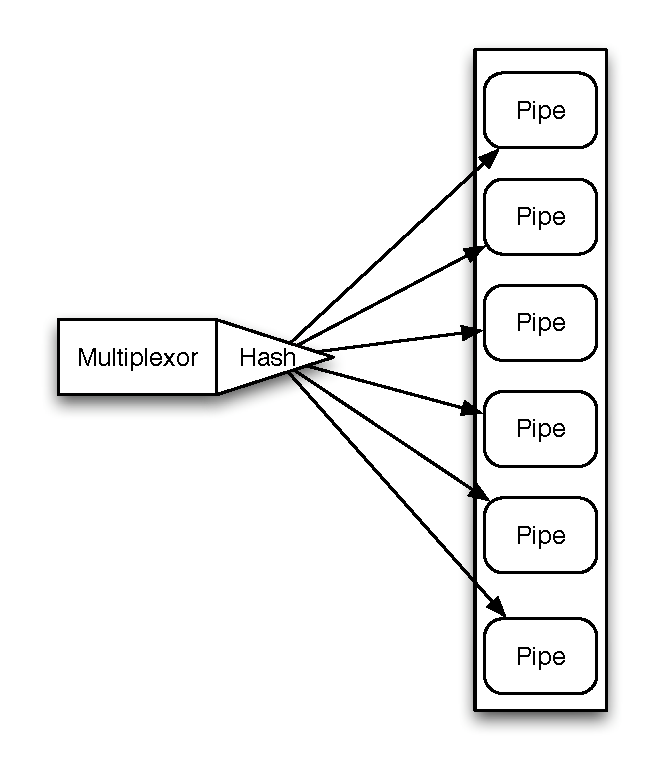
\includegraphics[width=2.0in]{mux.eps}
\caption{A Push Multiplexor. Push uses multiplexor modules to parse shell output into records and distributes those records according to a method implemented in the module}\label{fig:mux}
\end{figure}
Multiplexor modules expose an interface which provides Push with the ability to determine the desired record boundaries upon which to split the output data. The different modules are implemented as a set of filter requests asking for buffers of bytes. The shell provides these buffers by reading from a pipe attached to the standard output of the multiplexing program. Once these buffers have been provided the multiplexor module splits the data and then determines which of pipe of a multipipe to write to. The choice of which multipipe to target is left as a decision to the module. Different data formats may have different output requirements. For our main module, which operates on string values we use a djb2 hash to choose the target pipe and separate records on newline boundaries.

\begin{figure}[htp]
\centering
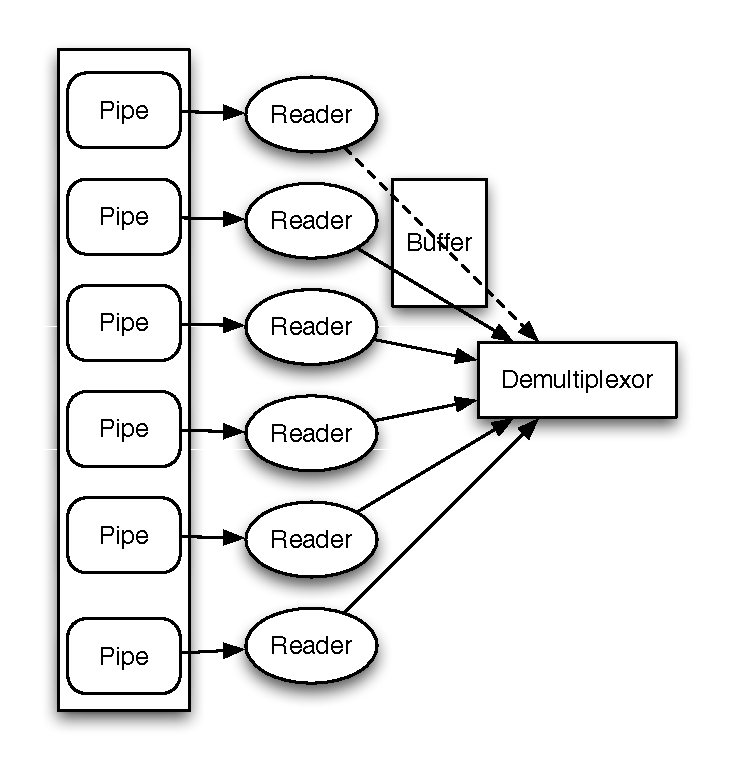
\includegraphics[height=2.0in]{demux.eps}
\caption{A Push Demultiplexor. Push Demultiplexors spawn reader threads for each pipe in a multipipe. These readers then pass buffer handles over a channel to the Demultiplexor which writes them to an output pipe}\label{fig:demux}
\end{figure}
Demultiplexing from a multipipe is performed by creating a many to one communications channel within the shell. The shell creates a reader processes which connect to each pipe in the multipipe. When the data reaches an appropriate record boundary a buffer is passed from the reader to the shell which then writes each record buffer to the output pipeline. 

This description leaves out one important caveat, how does the shell handle data that overruns buffer boundaries? In our current implementation of a multiplexor module the multiple reading operation is done by keeping a table of buffers which match the number of pipes in a multipipe. In the event that a buffer overflow(i.e. a record is too large for the buffer) the buffer table coalesces buffers until a complete record is obtained. In the event of buffer underflow(i.e. there are leftovers after every record in the buffer is consumed) the system attempts keeps the leftover buffer and appends it to the start of the next one, ensuring record continuity. This behavior has an effect on performance which is mentioned in the Performance section. 

\section{Push language overview}

To implement push we extended an existing shell, mash\cite{mashman}, from which we inherited a rich interpreted scripting language. Push functions much like traditional shells with the added goal of distributing computation over pipelines in order to make implementing DISC workflows easier. 

Push inherits its shell behavior from mash(1), it treats variables as lists of strings and has no native handling for any other data type. Integer expression handling and other facilities are provided by shell commands. It has native regular expression support and it has a novel ability to do declarative shell programming through a make like syntax incorporated in the shell itself.

Push differs from traditional shells by implementing native support for records based input handling over pipelines. This facility is similar to the argument field separators, IFS and OFS, in traditional shells which use a pattern to determine how to tokenize arguments. Push provides two variables, ORS and IRS, which point to record separator modules. These modules(called multiplexors in push) split data on record boundaries,  emitting individual records that the system distributes and coalesces. 

Multiplexors can be instantiated through the use of two types of multi-pipes, a multiplexing fan-out(\verb!|<!)  which distributes records to a set of pipes and a demultiplexing fan-in(syntax \verb!>|!) which coalesces records from a multipipe. This combination allows push to distribute IO to and from multiple simultaneous threads of control. The system defaults to separating records based on newlines, although an xml multiplexor is available and more will be available in the future. 
\subsection{Fanning in and Fanning out}

\begin{figure}[htp]
\centering
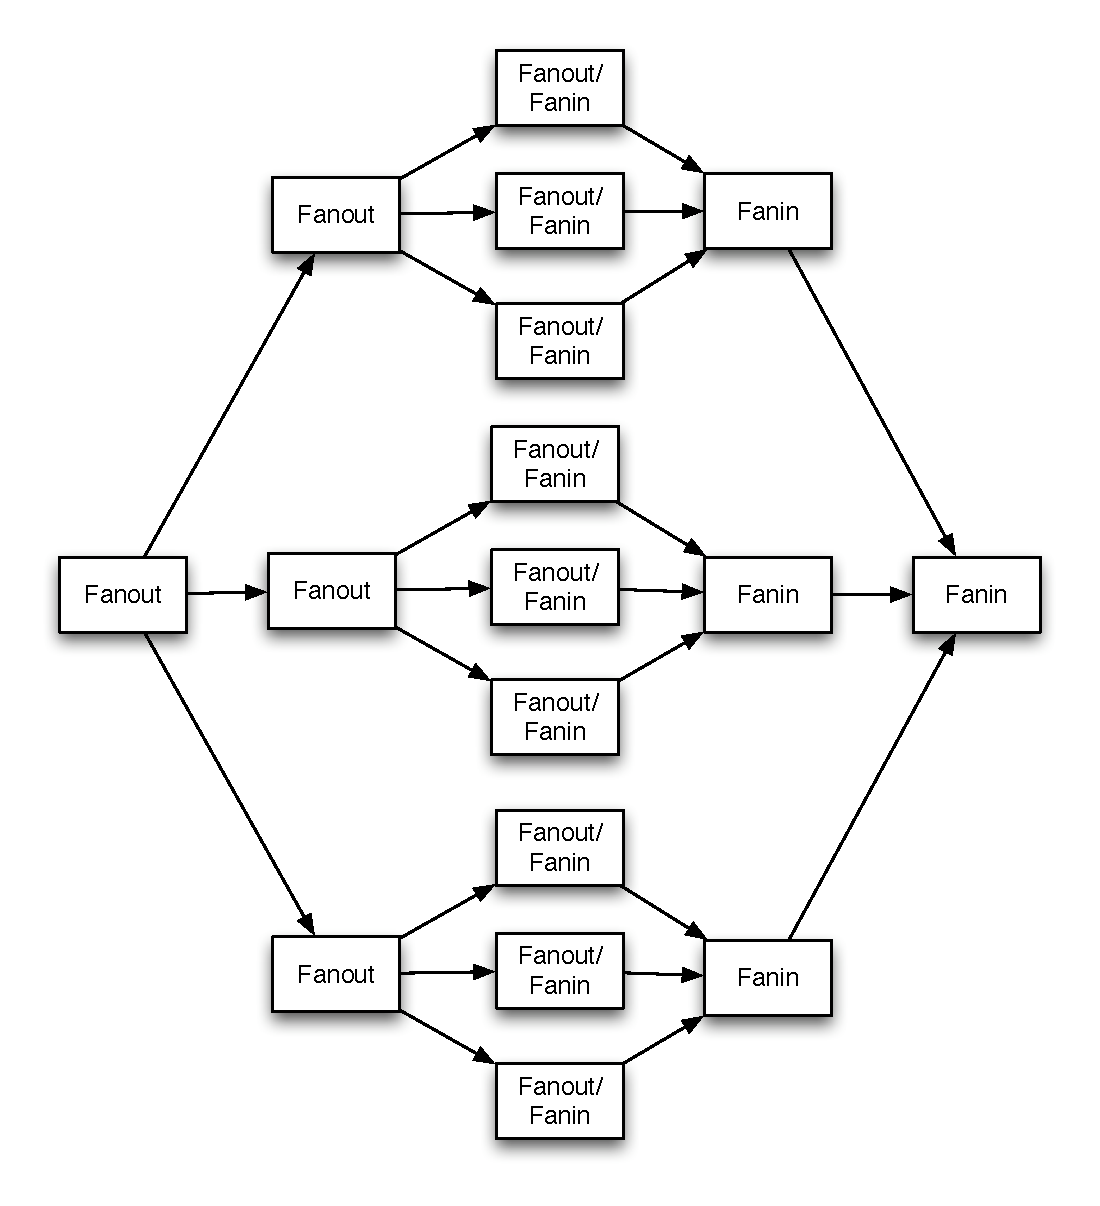
\includegraphics[height=2.5in]{fofigraph.eps}
\caption{Fan out and Fan in can be used to create arbitrary graphs of threads of control. Each fan out output node is capable of spawning more fan outs, which are then resolved by cascading fan ins}\label{fig:fofigraph}
\end{figure}

Push's novelty comes from its ability to create arbitrary acyclic graphs of distributed processes at the shell level. Users begin by fanning out some data which goes to the standard input of a set of processes. Figure ~\ref{fig:fofigraph} shows an example of this type of graph creation.

Based on an understanding of this ability to generate communications graphs, Push programs normally take some initial data source, e.g. a list of filenames or a set of records in a file, and then distributes input new threads of control potentially on a remote system.  When this data is distributed then the new program instantiate themselves they also have the ability to fan out and fan in arbitrary subgraphs as well. 

Since each fan in is matched to a fan out the graphs gradually coalesce until the output merges into one stream writing to the originating standard output. 

This matching of the first fan out to the last fan in gives multipipes similar semantics to parentheses. They can been seen as a grouping structure, binding the statements occuring between each multipipe to a set of new threads of control. This precedence order can be manually overridden by creating groups of processes using mash's shell groups(delimited with brackets '\{' and '\}').
\section{Resource conservation and understanding distribution}

Because push can potentially spawn many threads of control running on different machines push can potentially be very expensive to run. To avoid this problem push provides facilities that let users prototype their scripts before executing them on a potentially huge system. 

Push provides two facilities to solve this problem:

First, users can specify resource limits using the '-p' flag. This second argument to this flag specifies the maximum size of a multipipe, limiting the user to what they can do.

Second,  push provides a '-g' flag which aid in the debugging of the distribution of shell scripts. '-g' outputs the composition of a push script as a directed graph in dot\cite{koutsofios1999dgd} format. This allows users to view how their computation will be distributed between threads, allowing them to check their scripts for potential distribution errors. 
\section{Performance}

\subsection{Pipeline instantiation}

To test the effects of our multipipe infrastructure compared to a regular shell we wrote a shell script which explicitly dictates the size of the multipipes given to push and then instantiated a simple filter which passed its output unmodified through a pipe, with the goal of testing how long it takes to instantiate and use multipipes. Table ~\ref{fig:mpipeohead} shows these results.
\begin{figure}[htp]
\centering
\begin{center}

  \begin{tabular}{ | c | c | c || c |}
 \hline
 \# pipes & System Time & User Time & Total Time \\
 \hline
 1 & 0.001l & 0.009r & 0.01t \\
 2 & 0.002l & 1.278r & 1.28t \\ 
 4 & 0.002l & 1.239r & 1.241t \\
 8 & 0.001l & 1.195r & 1.196t \\
 16 & 0l & 1.146r & 1.146t \\
32 & 0l & 1.084r & 1.084t \\
64 & 0.001l & 1.077r & 1.078t \\
128 & 0.001l & 1.103r & 1.104t \\
 256 & 0.001l & 1.032r & 1.033t \\
 512 & 0l & 1.061r & 1.061t \\
 1024 & 0.001l & 1.026r & 1.027t \\
 2048 & failed & failed & failed \\
 \hline
 \end{tabular}
\end{center}
\caption{Overhead for multipipe reading and writing on a single machine}\label{fig:mpipeohead}
\end{figure}

The results of this show that the main bottleneck is the record handling in our pipe multiplexing, specifically the handling of left over records. Performance actually \emph{improves} as the number of pipes increases, which is counterintuitive. We believe this poor performance is due to the constant hammering of small record writes to each pipe. When the data is distributed over a large swath of pipes we have fewer problems with waiting for blocking reads. In the future we intend to explore this behavior more fully and optimize this behavior.

\subsection{IO Bound tasks}

(Note to editor, task evaluation is currently underway and will be available for the Camera ready)


\subsection{CPU bound tasks}

(Note to editor, task evaluation is currently underway and will be available for the Camera ready)     

\section{Future Work}
 
Right now Push is a useful tool for creating ad hoc solutions to DISC problems but it has difficulty handling programs that don't adhere to standard UNIX IO practices. 

Many modern UNIX programs, especially research tools, do not support writing to standard in and standard out. For example many Natural Language Processing tools that add annotation to documents expect and input and ouput file. This limits the efficacy of push, which relies on programs which read and write standard input. Tools written for push need to be very careful to read from standard input and write to standard output as default behaviors.

Likewise because push distributes streaming data over potentially remote links push is prone to causing network congestion between nodes. Tools that better preserve data locality like Plan 9's cfs(a caching user level filesystem) and a distributed databases similar to Google's Bigtable\cite{chang2006bds} manipulated by queries over multipipes would better preserve the locality of data. 

In addition to locality of data, Push could better preserve locality of computation  if its underlying operating system Inferno supported multiple cores.  Multicore support in Inferno's OS would allow local distribution of tasks as well as better threading supporting for push's subtasks(like multiplexors).

Push needs wider coverage of modules over different file formats. A way of passing arguments to multiplexor modules would also be very useful. For example a multiplexor xml module that supported XPath\cite{clark1999xpl} could be very useful for extracting relevant chunks of data from an xml file and then post processing them with UNIX tools.       


Finally it can cost a lot of money to use Push if you are using a system like EC2. Naive users can conceivably unknowingly spend large amounts of money using an incorrect push invocation. Some way of setting limits to the amount of systems/resource time used by a push invocation would better allow push to protect users from mistakes other than the -p and -g options would be useful. 
\section{Conclusion}

With the advent of a variety of utility computing systems users have the ability to create their own clusters of machines. However the ability to quickly and easily use these clusters doesn't exist yet. Users must use predefined workflows or high level languages to solve DISC problems.

We presented Push, a shell designed to solve DISC problems. Push reduces the complexity of instantiating and provisioning computation as well as distributing output in a way that conforms to and extends the traditional way UNIX way of distributing commands. Users can chain a variety of preexisting UNIX tools together unmodified, combining compiled programs, domain specific languages and shell scripts to solve pressing tasks.

This allows users to take advantage of their ability to create their own ad hoc DISC systems, giving users the greater flexibility than static middleware based approaches. 

\section{Acknowledgements}
 
I would like to thank Sape Mullender and James Mckie from Bell Labs for giving me feedback and advice on the construction of Push. Bruce Ellis took the time to explain the original goals and design of mash. Jonathan Appavoo and Amos Waterland helped me set up Kittyhawk and answering my questions.  Jordi Polo and William Polensky helped proofread this paper and offered formatting advice. I would like to thank my advisor Masayuki Asahara for advice and support. This work has been supported by the Department of Energy Of Office of Science Operating and Runtime Systems for Extreme Scale Scientific Computation project under contract \#DE-FG02-08ER25851. We have also benefited from access to the Argonne National Lab Blue Gene/P as part of the Department of Energy INCITE program.



\bibliographystyle{plain}

\bibliography{thesis}

\end{document}






